\documentclass[14pt]{article}

\usepackage{amsmath,amsthm,amssymb}
%%%%% Matrix stretcher
% use it as:
%\begin{pmatrix}[1.5]
% ...
\makeatletter
\renewcommand*\env@matrix[1][\arraystretch]{%
  \edef\arraystretch{#1}%
  \hskip -\arraycolsep
  \let\@ifnextchar\new@ifnextchar
  \array{*\c@MaxMatrixCols c}}
\makeatother
%%%%%%%%%%%%%%%%%%%%%%%%%%
\newcommand\extrafootertext[1]{%
    \bgroup
    \renewcommand\thefootnote{\fnsymbol{footnote}}%
    \renewcommand\thempfootnote{\fnsymbol{mpfootnote}}%
    \footnotetext[0]{#1}%
    \egroup
}


% Colors
\usepackage[dvipsnames]{xcolor}

\definecolor{C0}{HTML}{1d1d1d}
\definecolor{C1}{HTML}{1e3668}
\definecolor{C2}{HTML}{199d8b}
\definecolor{C3}{HTML}{d52f4c}
\definecolor{C4}{HTML}{5ab2d6}
\definecolor{C5}{HTML}{ffb268}
\definecolor{C6}{HTML}{ff7300} % for commenting - {fire orange}dd571c
\definecolor{C7}{HTML}{777b7e} % for remarks - {steel grey}
\color{C0}
%
% fonts
\usepackage[no-math]{fontspec}

\emergencystretch=8pt
\hyphenpenalty=1000 % default 50
\tolerance=800      % default 200
%\righthyphenmin=4
%\lefthyphenmin=4

\setmainfont[
    BoldFont = Vollkorn-Bold,
    ItalicFont = Vollkorn-Italic,
    BoldItalicFont={Vollkorn-BoldItalic},
    RawFeature=+lnum,
]{Vollkorn}
\newfontfamily\myfont{Copperplate-Gothic-Bold-Regular}% not good, sad
\usepackage[scale=.78]{luatexja-fontspec}
\setmainjfont{BabelStone Han}[AutoFakeBold]

% This package simplifies the insertion of external multi-page PDF or PS doc- uments.
\usepackage{pdfpages}

% cref
\usepackage{hyperref}
\hypersetup{
    colorlinks=true,
    linkcolor=C4,
    filecolor=magenta,      
    urlcolor=cyan,
    }

\usepackage[nameinlink,noabbrev,capitalize]{cleveref}
% \crefname{ineq}{}{}
% \crefname{equation}{}{}
% \creflabelformat{ineq}{#2{\textup{(1)}}#3}
% \creflabelformat{equation}{#2\textup{(#1)}#3}

% theorem-like environment
\newtheorem{theorem}{Theorem}[section]
\newtheorem{assumption}[theorem]{Assumption}
\newtheorem{lemma}[theorem]{Lemma}
\newtheorem{corollary}[theorem]{Corollary}
\newtheorem{proposition}[theorem]{Proposition}
\newtheorem{property}[theorem]{Property}

\newtheorem{definition}[theorem]{Definition}

\theoremstyle{definition}
\newtheorem{example}[theorem]{Example}
\newtheorem{problem}[theorem]{Problem}

% framed package is great
\usepackage{framed}
\newenvironment{solution}
{\color{C2}\begin{framed}\begingroup\textbf{Solution:} }
  {\endgroup\end{framed}}

\newtheoremstyle{remark}% name of the style to be used
  {}% measure of space to leave above the theorem. E.g.: 3pt
  {}% measure of space to leave below the theorem. E.g.: 3pt
  {\color{C3}}% name of font to use in the body of the theorem
  {}% measure of space to indent
  {\color{C3}\bfseries}% name of head font
  {.}% punctuation between head and body
  { }% space after theorem head; " " = normal interword space
  {}
\theoremstyle{remark}
\newtheorem{remarkx}[theorem]{Remark}
\newenvironment{remark}
  {\pushQED{\qed}\renewcommand{\qedsymbol}{$\triangle$}\remarkx}
  {\popQED\endremarkx}
  
\newenvironment{point}
  {\O~~}
  {}

\usepackage{thmtools}
\usepackage{thm-restate}
\usepackage{multicol}


% Page Formatting
\usepackage[
    paper=a3paper,
    inner=22mm,         % Inner margin
    outer=22mm,         % Outer margin
    bindingoffset=0mm, % Binding offset
    top=28mm,           % Top margin
    bottom=22mm,        % Bottom margin
    %showframe,         % show how the type block is set on the page
]{geometry}

\setlength{\parindent}{0em}
\setlength{\parskip}{.7em}


\usepackage{tikz}
\usepackage{graphicx}
\usepackage{enumitem}
\setlist{topsep=0pt}

\usepackage{bm}
\usepackage{extarrows} % \xlongequal{xxx}


\usepackage[font=scriptsize,labelfont=bf]{caption}
\usepackage{listings}
\lstset{basicstyle=\ttfamily,breaklines=true}
% \setlength{\parskip}{1em}
% \setlength{\parindent}{0em}
\usepackage{dsfont}
\newcommand{\bOne}{\mathds{1}}
\newcommand{\PP}{\mathbb{P}}
\newcommand{\EE}{\mathbb{E}}
\newcommand{\VV}{\mathbb{V}}
\newcommand{\CoV}{\operatorname{Co\mathbb{V}}}

% header
\usepackage{fancyhdr}
\pagestyle{fancy}
\fancyhead{}
\fancyhead[L]{\small   \bfseries Quant Review}
\fancyhead[C]{\small   \bfseries Fall 2022}
\fancyhead[R]{\small   \bfseries Zhou}





\begin{document}



\begin{center}
    \title{Quant Review}
    \text{\Large{Calculus and Linear Algebra
        }}

    {\text{Kaiwen Zhou}}


\end{center}

\tableofcontents
\newpage

\vspace{2em}


\section{Calculus}
\begin{theorem} Taylor Expansion
    \[f(x) = T_n(x) + R_n(x) = \sum_{i=0}^{n} \frac{f^{(i)}(a)}{i!}(x-a)^i + \frac{f^{(n+1)}(\xi)}{(n+1)!}(x-a)^{n+1}, \quad \text{for some} \quad\xi\in [a, x]\]
    where we must have $\lim_{n\to \infty} R_n(x) = 0$.

    We use $T_n(x)=\sum_{i=0}^{n} \frac{f^{(i)}(a)}{i!}(x-a)^i$ as the approximate for $f(x)$, and $R_n(x)= \frac{f^{(n+1)}(\xi)}{(n+1)!}(x-a)^{n+1}$ as the error of approximation.

    The bound for the remainder $R_n(x)$ is $|R_n(x)| \le \frac{M}{(n+1)!}(x-a)^{n+1}$, $M = \max_{\xi\in[a,x]} |f^{(n+1)}(\xi)|$.
\end{theorem}
\begin{lemma}\label{lemma:Useful Lemma for Differentiating Integrals}\textbf{(Useful Lemma for Differentiating Integrals)}
    Let $p(x)=\int_x^C f(u) d u$ and $q(x)=\int_C^x f(u) d u$, where $C$ a constant, it is easy to verify the following.
    $$
        \frac{d}{d x} p(x)=-f(x), \quad \frac{d}{d x} q(x)=f(x)
    $$
\end{lemma}

\subsection{Leibniz integral rule}
\begin{theorem}\textbf{(Leibniz integral rule)}
    In calculus, the Leibniz integral rule for differentiation under the integral sign states that for an integral of the form
    $$
        \int_{a(x)}^{b(x)} f(x, t) d t
    $$
    where $-\infty<a(x), b(x)<\infty$ and the integrands are functions dependent on $x$, the derivative of this integral is expressible as
    $$
        \frac{d}{d x}\left(\int_{a(x)}^{b(x)} f(x, t) d t\right) =f(x, b(x)) \cdot \frac{d}{d x} b(x)-f(x, a(x)) \cdot \frac{d}{d x} a(x)+\int_{a(x)}^{b(x)} \frac{\partial}{\partial x} f(x, t) d t
    $$
    where the partial derivative $\frac{\partial}{\partial x}$ indicates that inside the integral, only the variation of $f(x, t)$ with $x$ is considered in taking the derivative.
\end{theorem}

\begin{solution}
    This comes straightaway from Leibniz rule and Chain rule. Let
    $$
        g(x, a(x), b(x))=\int_{a(x)}^{b(x)} f(t, x) d t
    $$
    Using the Chain rule of integration
    $$
        \begin{aligned}
            \frac{d}{d x} g(x, a(x), b(x))                                         & =\frac{\partial g}{\partial x}  \frac{d x}{d x}+\frac{\partial g}{\partial a} \frac{d a}{d x}+\frac{\partial g}{\partial b} g \frac{d b}{d x} \\
            \cref{lemma:Useful Lemma for Differentiating Integrals}\Longrightarrow & =\int_{a(x)}^{b(x)} \frac{\partial}{\partial x} f(t, x) d t-f(a(x), x) \frac{d}{d x} a(x)+f(b(x), x) \frac{d}{d x} b(x)
        \end{aligned}
    $$
\end{solution}
\begin{remark}\hfill
    \begin{enumerate}
        \item When applying the \cref{lemma:Useful Lemma for Differentiating Integrals} in the above proof, we treat $b(x)$ and $a(x)$ as constants when doing $\frac{\partial g}{\partial a}$ and $\frac{\partial g}{\partial b}$ respectively.
        \item In the special case where the functions $a(x)$ and $b(x)$ are constants $a(x)=a$ and $b(x)=b$ with values that do not depend on $x$, this simplifies to:
              $$
                  \frac{d}{d x}\left(\int_a^b f(x, t) d t\right)=\int_a^b \frac{\partial}{\partial x} f(x, t) d t
              $$
        \item If $a(x)=a$ is constant and $b(x)=x$, which is another common situation (for example, in the proof of Cauchy's repeated integration formula), the Leibniz integral rule becomes:
              $$
                  \frac{d}{d x}\left(\int_a^x f(x, t) d t\right)=f(x, x)+\int_a^x \frac{\partial}{\partial x} f(x, t) d t
              $$
    \end{enumerate}
\end{remark}
\begin{problem}
We have the integral equation
$$
    \int_0^x\left(1+x+e^{x-t}\right) y(t) \mathrm{d} t=g(x), \quad 0 \leq x \leq 1
$$
By using Leibniz integral rule, we have that
$$
    g^{\prime}(x)=(2+x) y(x)+\int_0^x\left(1+e^{x-t}\right) y(t) \mathrm{d} t
$$
Where $y$ and $g$ are chosen to satisfy the condition of Leibniz integral rule.
\end{problem}
\begin{solution}
    In the above example, $a(x)=0, b(x)=x, f(t, x)=\left(1+x+e^x e^{-t}\right) y(t)$, we will have the above equation simplifies to,
    \begin{align*}
        \frac{d}{d x} g\left(x,a(x),b(x) \right) = & \int_{a(x)}^{b(x)}{\frac{\partial}{\partial x} f(t,x) dt }  - f\left(a(x),x\right) \frac{d}{d x} a(x) +  f\left(b(x),x\right) \frac{d}{d x} b(x) \\
        =                                          & \int_{0}^{x}{\frac{\partial}{\partial x} \left( 1+x+ e^{x}  e^{-t} \right) y(t)   dt }  - \left(1+x+ e^{x}  e^{0} \right) y(0)   \frac{d}{d x} 0 \\
                                                   & \quad +  \left(1+x+ e^{x}  e^{-x}\right) y(x)   \frac{d}{d x} x                                                                                  \\
        =                                          & \int_{0}^{x}{ \left( 1+ e^{x}  e^{-t} \right) y(t)   dt }+  \left(1+x +1\right) y(x)                                                             \\
        =                                          & \left(2+x\right) y(x) +   \int_{0}^{x}{ \left( 1+ e^{x-t}  \right) y(t)   dt }.
    \end{align*}
\end{solution}

\subsection{Gradient}

\subsection{Jacobian Matrix}
Suppose $\mathbf{f}: \mathbf{R}^n \rightarrow \mathbf{R}^m$ is a function such that each of its first-order partial derivatives exist on $\mathbf{R}^n$. This function takes a point $\mathbf{x} \in \mathbf{R}^n$ as input and produces the vector $\mathbf{f}(\mathbf{x}) \in \mathbf{R}^m$ as output. Then the Jacobian matrix of $\mathbf{f}$ is defined to be an $m \times n$ matrix, denoted by $\mathbf{J}$, whose $(i, j)$ th entry is $\mathbf{J}_{i j}=\frac{\partial f_i}{\partial x_j}$, or explicitly
$$
    \mathbf{J}=\left[\begin{array}{ccc}
            \frac{\partial \mathbf{f}}{\partial x_1} & \cdots & \frac{\partial \mathbf{f}}{\partial x_n}
        \end{array}\right]=\left[\begin{array}{c}
            \nabla^{\mathrm{T}} f_1 \\
            \vdots                  \\
            \nabla^{\mathrm{T}} f_m
        \end{array}\right]=\left[\begin{array}{ccc}
            \frac{\partial f_1}{\partial x_1} & \cdots & \frac{\partial f_1}{\partial x_n} \\
            \vdots                            & \ddots & \vdots                            \\
            \frac{\partial f_m}{\partial x_1} & \cdots & \frac{\partial f_m}{\partial x_n}
        \end{array}\right]
$$
where $\nabla^{\mathrm{T}} f_i$ is the transpose (row vector) of the gradient of the $i$ component.
The Jacobian matrix, whose entries are functions of $\mathbf{x}$, is denoted in various ways; common notations include $ D \mathbf{f}, \mathbf{J}_{\mathbf{f}}, \nabla \mathbf{f}$, and $\frac{\partial\left(f_1, \ldots, f_m\right)}{\partial\left(x_1, \ldots, x_n\right)}$. Some authors define the Jacobian as the transpose of the form given above.

\textbf{Example 1}
Consider the function $\mathbf{f}: \mathbf{R}^2 \rightarrow \mathbf{R}^2$, with $(x, y) \mapsto\left(f_1(x, y), f_2(x, y)\right)$, given by
$$
    \mathbf{f}\left(\left[\begin{array}{l}
            x \\
            y
        \end{array}\right]\right)=\left[\begin{array}{l}
            f_1(x, y) \\
            f_2(x, y)
        \end{array}\right]=\left[\begin{array}{c}
            x^2 y \\
            5 x+\sin y
        \end{array}\right] .
$$
Then we have
$$
    f_1(x, y)=x^2 y
$$
and
$$
    f_2(x, y)=5 x+\sin y
$$
and the Jacobian matrix of $\mathbf{f}$ is
$$
    \mathbf{J}_{\mathbf{f}}(x, y)=\begin{bmatrix}[1.5]
        \frac{\partial f_1}{\partial x} & \frac{\partial f_1}{\partial y} \\
        \frac{\partial f_2}{\partial x} & \frac{\partial f_2}{\partial y}
    \end{bmatrix}=\left[\begin{array}{cc}
            2 x y & x^2    \\
            5     & \cos y
        \end{array}\right]
$$
and the Jacobian determinant is
$$
    \\det\left(\mathbf{J}_{\mathbf{f}}(x, y)\right)=2 x y \cos y-5 x^2
$$

\textbf{Example 2:} polar-Cartesian transformation [ edit]
The transformation from polar coordinates $(r, \varphi)$ to Cartesian coordinates $(x, y)$, is given by the function $\mathbf{F}: \mathbf{R}^{+} \times[0,2 \pi) \rightarrow \mathbf{R}^2$ with components:
$$
    \begin{aligned}
         & x=r \cos \varphi                                                                                        \\
         & y=r \sin \varphi                                                                                        \\
         & \mathbf{J}_{\mathbf{F}}(r, \varphi)=\begin{bmatrix}[1.5]
                                                   \frac{\partial x}{\partial r} & \frac{\partial x}{\partial \varphi} \\
                                                   \frac{\partial y}{\partial r} & \frac{\partial y}{\partial \varphi}
                                               \end{bmatrix}=\left[\begin{array}{cc}
                                                                           \cos \varphi & -r \sin \varphi \\
                                                                           \sin \varphi & r \cos \varphi
                                                                       \end{array}\right]
    \end{aligned}
$$
The Jacobian determinant is equal to $r$. This can be used to transform integrals between the two coordinate systems:
$$
    \iint_{\mathbf{F}(A)} f(x, y) d x d y=\iint_A f(r \cos \varphi, r \sin \varphi) r d r d \varphi .
$$

\textbf{Example 3:} spherical-Cartesian transformation [ edit ]
The transformation from spherical coordinates $(r, \varphi, \theta)^{[6]}$ to Cartesian coordinates $(x, y, z)$, is given by the function $\mathbf{F}: \mathbf{R}^{+} \times[0, \pi) \times[0,2 \pi) \rightarrow \mathbf{R}^3$ with components:
$$
    \begin{aligned}
         & x=r \sin \varphi \cos \theta ; \\
         & y=r \sin \varphi \sin \theta ; \\
         & z=r \cos \varphi .
    \end{aligned}
$$
The Jacobian matrix for this coordinate change is
$$
    \mathbf{J}_{\mathbf{F}}(r, \varphi, \theta)=\begin{bmatrix}[1.5]
        \frac{\partial x}{\partial r} & \frac{\partial x}{\partial \varphi} & \frac{\partial x}{\partial \theta} \\
        \frac{\partial y}{\partial r} & \frac{\partial y}{\partial \varphi} & \frac{\partial y}{\partial \theta} \\
        \frac{\partial z}{\partial r} & \frac{\partial z}{\partial \varphi} & \frac{\partial z}{\partial \theta}
    \end{bmatrix}=\left[\begin{array}{ccc}
            \sin \varphi \cos \theta & r \cos \varphi \cos \theta & -r \sin \varphi \sin \theta \\
            \sin \varphi \sin \theta & r \cos \varphi \sin \theta & r \sin \varphi \cos \theta  \\
            \cos \varphi             & -r \sin \varphi            & 0
        \end{array}\right]
$$
The determinant is $r^2 \sin \varphi$. Since $d V=d x d y d z$ is the volume for a rectangular differential volume element (because the volume of a rectangular prism is the product of its sides), we can interpret $d V=r^2 \sin \varphi d r d \varphi d \theta$ as the volume of the spherical differential volume element. Unlike rectangular differential volume element's volume, this differential volume element's volume is not a constant, and varies with coordinates $(r$ and $\varphi)$. It can be used to transform integrals between the two coordinate systems:
$$
    \iiint_{\mathbf{F}(U)} f(x, y, z) d x d y d z=\iiint_U f(r \sin \varphi \cos \theta, r \sin \varphi \sin \theta, r \cos \varphi) r^2 \sin \varphi d r d \varphi d \theta
$$

\textbf{Example 4:}
The Jacobian matrix of the function $\mathbf{F}: \mathbf{R}^3 \rightarrow \mathbf{R}^4$ with components
$$
    \begin{aligned}
         & y_1=x_1           \\
         & y_2=5 x_3         \\
         & y_3=4 x_2^2-2 x_3 \\
         & y_4=x_3 \sin x_1
    \end{aligned}
$$
is
\[
    \mathbf{J}_{\mathbf{F}}\left(x_1, x_2, x_3\right)=\begin{bmatrix}[1.5]
        \frac{\partial y_1}{\partial x_1} & \frac{\partial y_1}{\partial x_2} & \frac{\partial y_1}{\partial x_3} \\
        \frac{\partial y_2}{\partial x_1} & \frac{\partial y_2}{\partial x_2} & \frac{\partial y_2}{\partial x_3} \\
        \frac{\partial y_3}{\partial x_1} & \frac{\partial y_3}{\partial x_2} & \frac{\partial y_3}{\partial x_3} \\
        \frac{\partial y_4}{\partial x_1} & \frac{\partial y_4}{\partial x_2} & \frac{\partial y_4}{\partial x_3}
    \end{bmatrix}=\left[\begin{array}{ccc}
            1            & 0     & 0        \\
            0            & 0     & 5        \\
            0            & 8 x_2 & -2       \\
            x_3 \cos x_1 & 0     & \sin x_1
        \end{array}\right] .
\]
This example shows that the Jacobian matrix need not be a square matrix.

\textbf{Example 5:}
The Jacobian determinant of the function $\mathbf{F}: \mathbf{R}^3 \rightarrow \mathbf{R}^3$ with components
$$
    \begin{aligned}
         & y_1=5 x_2                               \\
         & y_2=4 x_1^2-2 \sin \left(x_2 x_3\right) \\
         & y_3=x_2 x_3
    \end{aligned}
$$
is
$$
    \left|\begin{array}{ccc}
        0     & 5                                & 0                                \\
        8 x_1 & -2 x_3 \cos \left(x_2 x_3\right) & -2 x_2 \cos \left(x_2 x_3\right) \\
        0     & x_3                              & x_2
    \end{array}\right|=-8 x_1\left|\begin{array}{cc}
        5   & 0   \\
        x_3 & x_2
    \end{array}\right|=-40 x_1 x_2 .
$$
From this we see that $\mathbf{F}$ reverses orientation near those points where $x_1$ and $x_2$ have the same sign; the function is locally invertible everywhere except near points where $x_1=0$ or $x_2=0$. Intuitively, if one starts with a tiny object around the point $(1,2,3)$ and apply $\mathbf{F}$ to that object, one will get a resulting object with approximately $40 \times 1 \times 2=80$ times the volume of the original one, with orientation reversed.







\subsection{Hessian Matrix}

\subsection{Taylor Expansion}


\newpage
\section{Linear Algebra}
\begin{multicols}{2}

    \section{Basics}
    \begin{proposition}
        \begin{enumerate}
            \item $\alpha \vec{v}+\beta \vec{u}$ - linear combination.
            \item $\alpha \vec{a}$ - line; \quad  $\alpha \vec{a}+\beta b-$ plane; \quad $\alpha \vec{a}+\beta \vec{b}+8 \vec{c}-$ space.
        \end{enumerate}
    \end{proposition}


    \begin{proposition}$\vec{a}=\left(a_1, a_2, a_3\right), \vec{b}=\left(b_1, b_2, b_3\right)$.
        \begin{enumerate}
            \item $\vec{a} \cdot \vec{b}=a_1 b_1+a_2 b_2+a_3 b_3=\vec{b} \cdot \vec{a}=\vec{a}^{\top} b=\vec{b}^{\top} \vec{a}$
            \item $\|\vec{a}\|=\sqrt{a_1^2+a_2^2+a_3^2}$
            \item $\frac{\vec{a} \cdot \vec{b}}{\|a\|\|b\|}=\cos \theta$
            \item $|\vec{a} \cdot \vec{b}| \leq\|\vec{a}\|\|\vec{b}\|$ (Cauchy-Schwartz)
            \item if $\vec{a} \cdot \vec{b}=0 \Rightarrow \vec{a}, \vec{b}$ perpendicular $\Rightarrow\|\vec{a}\|^2+\|\vec{b}\|^2=\|\vec{a}-\vec{b}\|^2$.
            \item  unit vector: $\|\vec{a}\|=1=\frac{\vec{b}}{\|\vec{b}\|}$
            \item $\vec{a}^\top \vec{b}$ - inner product; $\vec{a} \vec{b}^\top$ - outer product
            \item $e_i^\top A = Row_i(A)$.
            \item lower triangular matrix $\cdot$ lower triangular matrix $=$ lower triangular matrix.
        \end{enumerate}
    \end{proposition}

    \begin{proposition}\hfill
        \begin{enumerate}
            \item Linearly independence: $\alpha \vec{a}+\beta \vec{b}+\gamma \vec{c}=\overrightarrow{0}$ only if $\alpha=\beta=\gamma=0$
            \item linearly dependence: $\exists(\alpha, \beta, \gamma) \neq(0,0,0)$ sit. $\alpha \vec{a}+\beta \vec{b}+\gamma \vec{c}=\overrightarrow{0}$.
            \item $\left[\begin{array}{lll}| & | & | \\ \vec{a} & \vec{b} & \vec{c}\\
             |      & | & |\end{array} \right]\left[\begin{array}{l}\alpha \\ \beta\\
                              \gamma\end{array}\right]=\vec{0} \Longrightarrow \begin{cases} \text{linearly independence} \Longrightarrow A-invertible. \\
                          \text{linearly dependence $A$ - singular (not invertible)}
                      \end{cases}$
        \end{enumerate}

    \end{proposition}

    \textbf{Matix Multiplication}
    \begin{itemize}
        \item $A B=A\begin{bmatrix}\vec{b}_1 & \vec{b}_2 & \vec{b}_3
                  \end{bmatrix}=\begin{bmatrix}\vec{A} \vec{b}_1 & A \overrightarrow{b_2} & A \overrightarrow{b_3}\end{bmatrix}$.
        \item $Row_i(AB)= A\cdot Row_i(B)$.
        \item $Row_i(AB)= Row_i(A)\cdot B$.
    \end{itemize}
    %%%%%%%%%%%%%%%%

    \section{Vector norms}
    A norm $\|\cdot\|: \mathbb{R}^{n} \rightarrow \mathbb{R}$ is a function satisfying the properties:

    \begin{itemize}
        \item $\|x\|=0$ if and only if $x=0$ (definiteness)

        \item $\|c x\|=|c|\|x\|$ for all $c \in \mathbb{R}$ (homogeneity)

        \item $\|x+y\| \leq\|x\|+\|y\|$ (triangle inequality)

    \end{itemize}

    Common examples of norms:

    \begin{itemize}
        \item $\|x\|_{1}=\left|x_{1}\right|+\cdots+\left|x_{n}\right| \quad$ (the 1-norm)

        \item $\|x\|_{2}=\sqrt{x_{1}^{2}+\cdots+x_{n}^{2}} \quad$ (the 2-norm / Euclidean norm)  -> default norm

        \item $\|x\|_{\infty}=\max _{1 \leq i \leq n}\left|x_{i}\right| \quad$ (max-norm)

    \end{itemize}


    % \begin{wrapfigure}{l}{0.2\textwidth}
    % \centering
    % 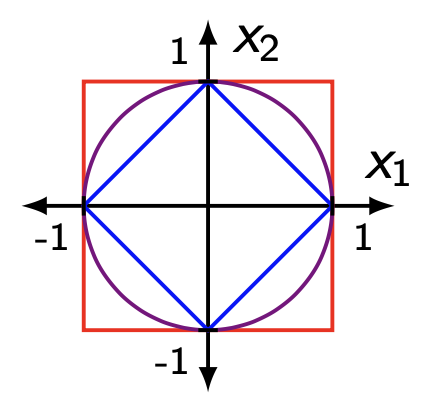
\includegraphics[width=0.2\textwidth]{norm ball.png}\caption{This is the Overleaf logo}
    % \end{wrapfigure}


\end{multicols}

\headrule

%%%%%%%%%%%%%%%%%%%%
\begin{multicols}{2}
    \section{Linear Equations, Elimination, Permutation}
    \textbf{Linear Equations}
    Given $A \in \mathbb{R}^{m \times n}$ and $b \in \mathbb{R}^{m}$, linear equations take the form
    \[
        A x=b
    \]
    where we must solve for $x \in \mathbb{R}^{n}$.

    \textbf{Understandings of $Ax = b$}
    \begin{itemize}
        \item $A \vec{x}$: matrix $A$ acts on $\vec{x}$.
        \item General Thinking: The column picture of $A \vec{x}=\vec{b}$.

              A combination of $n$ columns of $A$ produces the vector $\vec{b}$.

        \item Geometric Thinking: The row picture of $A \vec{x}=\vec{b}$ coefficient matrix

              Matrix $A$ can be view as a coefficient matrix, then $m$ equations from $m$ rows give $m$ planes ($P_i: \operatorname{row}_i \cdot \vec{x}-b_i=0$) meeting at $\vec{x}$.
    \end{itemize}

    \textbf{Four possibilities for solutions}
    \begin{itemize}
        \item $r=m=n \Longrightarrow R = \begin{bmatrix}
                      I
                  \end{bmatrix}$,  $A x=b$ has exactly one solution.
        \item $r=m, r<n \Longrightarrow R = \begin{bmatrix}
                      I & F
                  \end{bmatrix}$,  $A x=b$ has $\infty$ solution.
        \item $r<m, r=n \Longrightarrow R = \begin{bmatrix}
                      I \\
                      \bm{0}
                  \end{bmatrix}$,  $A x=b$ has $0$ or $1$ solution.

        \item $r<m, r<n \Longrightarrow R = \begin{bmatrix}
                      I      & F      \\
                      \bm{0} & \bm{0}
                  \end{bmatrix}$,  $A x=b$ has $0$ or $\infty$ solution.

    \end{itemize}

    \textbf{Idea of Elimination}

    The core idea is to convert $A$ to an upper Triangular matrix $A^{\prime}$ (Elimination), then solve for $\vec{x}$ from $x_n$ to $x_1$ (Back substitution). E.g.
    \[
        \underset{A}{\begin{bmatrix}
                * & * & * & * \\
                  & * & * & * \\
                  &   & * & * \\
                  &   &   & * \\
            \end{bmatrix}} \underset{x}{\begin{bmatrix}
                x_1 \\
                x_2 \\
                x_3 \\
                x_4
            \end{bmatrix}} = \underset{b}{\begin{bmatrix}
                b_1 \\
                b_2 \\
                b_3 \\
                b_4
            \end{bmatrix}}
    \]

    \textbf{Elimination matrix}
    $E_{ij}=\begin{bmatrix}
            1  &   &        &   \\
               & 1 &        &   \\
            -l &   & \ddots &   \\
               &   &        & 1
        \end{bmatrix}$ where $e_{ij} = -l$ is use to reduce the $(i, j)$ entry of $A$, $a_{ij}$, to zero.
    $$E_{ij} A=\begin{bmatrix}
            \vdots              \\
            Row_i-l \cdot Row_1 \\
            \vdots
        \end{bmatrix}, \quad E_{ij}^{-1} = \begin{bmatrix}
            1 &   &        &   \\
              & 1 &        &   \\
            l &   & \ddots &   \\
              &   &        & 1
        \end{bmatrix}
    $$

    \textbf{Permutation Matrix}

    $$
        P_{23}=\left[\begin{array}{lll}
                1 & 0 & 0 \\
                0 & 0 & 1 \\
                0 & 1 & 0
            \end{array}\right]=\left[\begin{array}{c}
                -{\vec{e_1}}^{\top}- \\
                -{\vec{e_3}}^{\top}- \\
                -{\vec{e_2}}^{\top}-
            \end{array}\right]
    $$
    $P_{23} A$ exchanges Row 2 \& Row 3 of matrix $A$.
    \begin{itemize}
        \item Permutation matrix is orthogonal matrix, i.e., $P^\top = P^{-1}, PP^\top = I$.
        \item Sometimes we need to exchange some rows of $A$ so it can be reduced to a valid rref $R$. In this case, we need permutation matrix $P$.

              E.g. $\begin{bmatrix}0 & 2  \\
               3 & -2
                  \end{bmatrix}$ can be fixed though has 0 as the first pivot
              $\Rightarrow\left[\begin{array}{cc}3 & -2 \\ 0 & 2\end{array}\right] \rightarrow$ a row exchange produces an upper triangular matrix.
        \item For the ease of Elimination \& Permutation for both sides of $A \vec{x}=\vec{b}$ we create an augmented matrix $L = \begin{bmatrix}A & \vec{b}\end{bmatrix}$ and let elimination and permutation matrices act on $L$.
              $$
                  \left(E_{i j} P_{i j} \cdots \right) \cdot\begin{bmatrix}A & \vec{b}\end{bmatrix}
              $$
    \end{itemize}

    \textbf{Pivots}
    \begin{itemize}
        \item Pivots are on the diagonal of the triangle after elimination.
              We need $n$ pivots to solve for $n$ unknowns.
    \end{itemize}

\end{multicols}
%%%%%%%%%%%%%%%%%%%%%%%%%%%%%%%%

\headrule

%%%%%%%%%%%%%%%%%%%%%%%%%%%%%%%%
\section{CR Decomposition}

%%%%%%%%%%%%%%%%%%%%%%%%%%%%%%%%

\headrule

%%%%%%%%%%%%%%%%%%%%%%%%%%%%%%%%
\section{LU Decomposition}


%%%%%%%%%%%%%%%%%%%%%%%%%%%%%%%%

\headrule

%%%%%%%%%%%%%%%%%%%%%%%%%%%%%%%%
\section{Inverse \& Transpose}
\begin{proposition}
    \textbf{(Basic properties of the matrix inverse and transpose): }

    \begin{tabular}{c|c|c}
        $A^{-1}$ is unique if it exists. & $\left(A^{-1}\right)^{-1}=A$     & $\left(A^{-1}\right)^{\top}=\left(A^{\top}\right)^{-1}$ \\\hline
        $(A B)^{-1}=B^{-1} A^{-1}$       & $\left(A^{\top}\right)^{\top}=A$ & $(A B)^{\top}=B^{\top} A^{\top}$
    \end{tabular}

    left-inverse = right inverse = two-sided inverse

    Suppose $B A=I$ \& $A C=I \Rightarrow B=B(A C)=(B A) C=C$.

    Gauss - Jordan Elimination for computing $A^{-1}$ By using $A^{-1}[A \mid I]=\left[I \mid A^{-1}\right]$
    where $[A \mid I]$ is the augmented matrix.
    $\Rightarrow$ convert $[A \mid I] \rightarrow[I \mid A]$ using elimination matrix.


\end{proposition}
\begin{figure}[!htp]
    \centering
    
\includegraphics[width=0.6\textwidth]{inverse.png}
    \caption{inverse all in one}
    \label{fig:enter-label}
\end{figure}


\headrule

%%%%%%%%%%%%%%%%%%%%%%%%%%%%%%%%
\begin{multicols}{2}
    \section{The rank of a matrix}

    Note: When considering rank, think about the rref (the row reduced echelon form) of a matrix.

    $\operatorname{rank}(A)=$ maximum number of linearly independent columns $=$ maximum number of linearly independent rows $=$ number of pivots

    If $A \in \mathbb{R}^{m \times n}$ and $B \in \mathbb{R}^{n \times p}$ then

    \begin{itemize}
        \item $\operatorname{rank}(A) \leq \min (m, n)$

        \item $\operatorname{rank}(A B) \leq \min (\operatorname{rank}(A), \operatorname{rank}(B)) \leq \min (m, n, p)$

        \item if $\operatorname{rank}(A)=n$ then $\operatorname{rank}(A B)=\operatorname{rank}(B)$

        \item if $\operatorname{rank}(B)=n$ then $\operatorname{rank}(A B)=\operatorname{rank}(A)$

    \end{itemize}

    So multiplying by an invertible matrix does not alter the rank.

    General properties of the matrix rank:

    \begin{itemize}
        \item $\operatorname{rank}(A+B) \leq \operatorname{rank}(A)+\operatorname{rank}(B)$

        \item $\operatorname{rank}(A)=\operatorname{rank}\left(A^{\top}\right)=\operatorname{rank}\left(A^{\top} A\right)=\operatorname{rank}\left(A A^{\top}\right)$

        \item $A \in \mathbb{R}^{n \times n}$ is invertible if and only if $\operatorname{rank}(A)=n$.
        \item rank-$1$ matrix $A = cuv^\top$ where $u\in\mathbb{R}^m$, $v\in\mathbb{R}^n$ and $A\in\mathbb{R}^{m\times n}$.
        \item rank-$2$ matrix $A = au_1v_1^\top + bu_2v_2^\top$ where $u_i\in\mathbb{R}^m$, $v_i\in\mathbb{R}^n$ and $A\in\mathbb{R}^{m\times n}$.
        \item rank-$k$ matrix $A = \sum_{i=1}^k a_iu_iv_i^\top$ where $u_i\in\mathbb{R}^m$, $v_i\in\mathbb{R}^n$ and $A\in\mathbb{R}^{m\times n}$.
    \end{itemize}

    \section{Four Spaces}
    \textbf{Vector Space:}

    \textbf{Subspace:}  $A$ is a subspace, $\subseteq$, of $S$ if $\forall u, v \in S, a, b$-constant, we have
    $au + bv \in S$.

    \textbf{Basis:} Vector spaces are linearly independent \& span the space. (e.g. The columns of every invertible matrix give a basis for $\mathbb{R}^n$.) The dimension of the space is the number of basis in the set of basis.

    \textbf{Four Space:} Given $A \in \mathbb{R}^{m \times n}$, we have the definitions:
    \begin{itemize}
        \item Range/Column/Image space: $R(A)=C(A)=Im(A)=\left\{A x \mid x \in \mathbb{R}^{n}\right\} \subseteq \mathbb{R}^{m}$.
        \item Row space: $C(A^\top)\subseteq \mathbb{R}^{n}$.
        \item Null/Kernel space: $N(A)=Ker(A)=\left\{x \in \mathbb{R}^{n} \mid A x=0\right\}\subseteq \mathbb{R}^{n}$.
        \item Left-Null space: $N(A^\top)=Ker(A^\top)=\left\{x \in \mathbb{R}^{m} \mid A^\top x=0\right\}\subseteq \mathbb{R}^{m}$.
    \end{itemize}
    \textbf{Properties:}
    \begin{itemize}
        \item The column space of $A \Longleftrightarrow$ the row space of $A^\top$.
        \item $0\in N(A)=Ker(A)$.
        \item Rank-Nullity Theorem: $\operatorname{rank}(A)+\operatorname{\dim}(N(A))=n$
        \item $\operatorname{\dim}(Im(A)) = \operatorname{\dim}(Im(A^\top)) = rank(A) = r$
        \item $\operatorname{\dim}(N(A)) = n - r$, $\operatorname{\dim}(N(A^\top)) = m - r$.
    \end{itemize}

    \textbf{Space Orthogonality:}
    The orthogonal complement of a subspace $V$, $V^\perp$, contains every vector that is perpendicular to $V$.
    \begin{itemize}
        \item $C(A^\top) = N(A)^\perp$, i.e. The row space is perpendicular to the null space. (Think $Ax = 0$.)
        \item $C(A) = N(A^\top)^\perp$, i.e. The column space is perpendicular to the null space of $A^\top$ (left-null space).(Think $A^\top x = 0$.)
        \item Suppose $A\in \mathbb{R}^{m\times n}$, $\forall x\in \mathbb{R}^n$, it can be represented as $x = x_r + x_n$ where $x_r \in C(A^\top)$ and $x_n \in N(A)$.
    \end{itemize}

    \textbf{rref of $A$:} Suppose $R= rref(A)$, then
    \begin{itemize}
        \item $C(A^\top) = C(R^\top)$, i.e.\ same row space.
        \item $C(A) \ne C(R)$, the lase few entries of $C(R)$ could only be zero.
        \item $\operatorname{\dim}(C(A)) = \operatorname{\dim}(C(R))$, ($Ax= 0 \Longrightarrow Rx = 0$).
        \item $N(A) = N(R)$.
    \end{itemize}

    \textbf{Link to equation $Ax=b$}

    The following statements are equivalent:
    \begin{itemize}
        \item There exists a solution to the equation $A x=b$.
        \item $b \in R(A)$.
        \item $\operatorname{rank}(A)=\operatorname{rank}\left(\left[\begin{array}{ll}A & b\end{array}\right]\right)$
    \end{itemize}

    The following statements are equivalent:
    \begin{itemize}
        \item Solutions to the equation $A x=b$ are unique.
        \item $N(A)=\{0\}$.
        \item $\operatorname{rank}(A)=n$.
    \end{itemize}
\end{multicols}
%%%%%%%%%%%%%%%%%%%%%%%%%%%%%%%

\headrule

%%%%%%%%%%%%%%%%%%%%%%%%%%%
\begin{multicols}{2}
    \section{Determinant}
    \begin{proposition}\textbf{(Basic 3)}\hfill
        \begin{enumerate}
            \item swapping two columns: $|\begin{bmatrix}
                          \cdots & \bm{a}_i & \cdots & \bm{a}_j & \cdots
                      \end{bmatrix}| = -|\begin{bmatrix}
                          \cdots & \bm{a}_j & \cdots & \bm{a}_i & \cdots
                      \end{bmatrix}|$
            \item $|\begin{bmatrix}
                          \cdots & \alpha\bm{u}+\beta\bm{v} & \cdots
                      \end{bmatrix}| = \alpha|\begin{bmatrix}
                          \cdots & \bm{u} & \cdots
                      \end{bmatrix}| + \beta|\begin{bmatrix}
                          \cdots & \bm{v} & \cdots
                      \end{bmatrix}|$
            \item duplicates: $|\begin{bmatrix}
                          \cdots & \bm{a}_i & \cdots & \bm{a}_i & \cdots
                      \end{bmatrix}| = 0$
        \end{enumerate}
    \end{proposition}

    \begin{proposition}
        If $A$ is singular $\Longleftrightarrow \{\bm{a}_1 \cdots \bm{a}_n\} ~\text{linearly dependent} \Longleftrightarrow  |A|=0$.
    \end{proposition}
    Hint: singular -> one of the columns / rows linearly depends on the rest -> use Basic 2 and 3.

    \begin{proposition}
        \begin{enumerate}
            \item $|I| = 1$, $|P^{permu}| = 1/-1$ (use Basic 1), $|P^{ortho}| = 1/-1$.
            \item $|A| = |A^\top|$
            \item $|AB| = |A|\cdot|B|$
            \item $|A^{-1}| = \frac{1}{|A|}$
            \item Orthogonal matrix $|Q|= \pm |1|$ because $Q^\top Q=I$ gives $|Q|^2=1$.
            \item Triangular matrix $|U|=u_{11} u_{22} \cdots u_{n n}$
            \item
                  $|A| = |L U|=|L|\cdot |U|=$ product of the pivots $u_{i i}$
            \item $\left|\begin{bmatrix}
                          A & 0 \\
                          0 & B \\
                      \end{bmatrix}\right| = |A|\cdot |B|$,$ \quad \left|\begin{bmatrix}
                          A & C \\
                          0 & B \\
                      \end{bmatrix}\right| = |A|\cdot |B|$.
        \end{enumerate}
    \end{proposition}
\end{multicols}
%%%%%%%%%%%%%%%%%%%%%%%%%%%

\headrule

\begin{proposition}
    \textbf{(Cramer's Rule)} Cramer's Rule to Solve $A x=b \quad$ Start from
    $$
        \left[\begin{array}{ll}
                \boldsymbol{A}
            \end{array}\right]\left[\begin{array}{lll}
                \boldsymbol{x}_{\mathbf{1}} & 0 & 0 \\
                \boldsymbol{x}_{\mathbf{2}} & 1 & 0 \\
                \boldsymbol{x}_{\mathbf{3}} & 0 & 1
            \end{array}\right]=\left[\begin{array}{lll}
                \boldsymbol{b}_{\mathbf{1}} & a_{12} & a_{13} \\
                \boldsymbol{b}_{\mathbf{2}} & a_{22} & a_{23} \\
                \boldsymbol{b}_{\mathbf{3}} & a_{32} & a_{33}
            \end{array}\right]=\boldsymbol{B}_{\mathbf{1}}
    $$
    Use $(\det \boldsymbol{A})\left(\boldsymbol{x}_1\right)=\left(\det \boldsymbol{B}_1\right)$ to find $\boldsymbol{x}_1$
    $\begin{array}{ll}\text { Same } \\ \text { idea }\end{array}[A]\left[\begin{array}{lll}1 & x_1 & 0 \\ 0 & x_2 & 0 \\ 0 & x_3 & 1\end{array}\right]=\left[\begin{array}{lll}a_1 & b & a_3\end{array}\right]=B_2 \quad \begin{aligned} & x_1=\frac{\det B_1}{\det A} \\ & x_2=\frac{\det B_2}{\det A}\end{aligned}$
    Cramer's Rule is usually not efficient! Too many determinants
    $$
        \left[\begin{array}{ll}
                3 & 2 \\
                5 & 4
            \end{array}\right]\left[\begin{array}{l}
                x_1 \\
                x_2
            \end{array}\right]=\left[\begin{array}{l}
                12 \\
                22
            \end{array}\right] \quad \boldsymbol{B}_1=\left[\begin{array}{ll}
                12 & 2 \\
                22 & 4
            \end{array}\right] \quad \boldsymbol{B}_2=\left[\begin{array}{ll}
                3 & 12 \\
                5 & 22
            \end{array}\right] \quad x_1=\frac{\det B_1}{\det A}=\frac{4}{2} \quad x_2=\frac{2}{2}
    $$
\end{proposition}

%%%%%%%%%%%%%%%%%%%%%%%%%%%

\headrule

%%%%%%%%%%%%%%%%%%%%%%%%%%%

\section{Least squares}
Suppose $A\in\mathbb{R}^{n\times p}$. When the linear equations $A x=b$ are overdetermined ($n>p$) and there is no solution, we minimize the 2-norm of the residual:
$$
    \underset{x}{\operatorname{minimize}}\|A x-b\|_{2} \Longrightarrow A^{\top} A \hat{x}=A^{\top} b \quad \rightarrow \text{Normal Equation}
$$
The normal equations have a unique solution iff $rank(A)=p$ (full column rank / the columns of $A$ are linearly independent). Why? Because $A^\top A \in \mathbb{R}^{p\times p}$ and $Im(A^\top A) = Im(A)\Longrightarrow rank(A^\top A) = rank(A) = p \Longrightarrow A^\top A$ is full rank.

Then,
$$
    \hat{x}=\left(A^{\top} A\right)^{-1} A^{\top} b = A^{\dagger} b
$$
where $A^{\dagger} = (A^\top A)^{-1}A^\top$ is the Moore-Penrose inverse (or pseudo-inverse).

%%%%%%%%%%%%%%%%%%%%%%%%%%%

\headrule

%%%%%%%%%%%%%%%%%%%%%%%%%%%
\begin{multicols}{2}

    \section{Orthogonal matrices}
    A square matrix $U$ is orthogonal if $U^{\top} U=I$.

    Some properties of orthogonal $U$ and $V$:
    \begin{itemize}
        \item \textbf{Orthogonal Columns and Rows}: $u_i\cdot u_j = 0$, $\|u_i\|=\|u_j\|=1$.

        \item \textbf{Orthogonal Basis}: The columns (or rows) of an orthogonal matrix form an orthogonal basis for the vector space.
        \item \textbf{Orthogonal transformations preserve angles \& length}: $(U x)^{\top}(U z)=x^{\top} z$ and $\|U x\|_{2}=\|x\|_{2}$.

        \item Certain matrix norms are also invariant: $\left\|U A V\right\|_{2}=\|A\|_{2}$ and $\left\|U A V\right\|_{F}=\|A\|_{F}$

        \item If $U$ is square, $U^{\top} U=U U^{\top}=I$ and $U^{-1}=U^{\top}$.

        \item $U V$ is orthogonal.

    \end{itemize}

    Every subspace has an orthonormal basis: For any $A \in \mathbb{R}^{m \times n}$, there exists an orthogonal $U \in \mathbb{R}^{m \times r}$ such that $R(A)=R(U)$ and $r=\operatorname{rank}(A)$. One way to find $U$ is using Gram-Schmidt.


    \columnbreak


    \section{Projections}
    If $P \in \mathbb{R}^{n \times n}$ satisfies $P^{2}=P$, $P^\top = P$ it's called a projection matrix.

    In general, $P: \mathbb{R}^{n} \rightarrow S$, where $S \subseteq \mathbb{R}^{n}$ is a subspace.

    If $P$ is a projection matrix, so is $(I-P)$. We can uniquely decompose:
    \[
        x=u+v = P x + (I-P) x \quad  \text { where } u \in S, v \in S^{\perp}
    \]
    Pythagorean theorem: $\|x\|_{2}^{2}=\|u\|_{2}^{2}+\|v\|_{2}^{2}$

    If $A \in \mathbb{R}^{m \times n}$ has linearly independent columns, then the projection onto $R(A)$ is given by $P=A\left(A^{\top} A\right)^{-1} A^{\top}$.
    \[e\perp R(A) \Longrightarrow (b-Ax)^\top A = 0 \Longrightarrow x = \left(A^{\top} A\right)^{-1} A^{\top} b \Longrightarrow p = Ax = A\left(A^{\top} A\right)^{-1} A^{\top}b\]

    Least-squares: decompose $b$ using the projection above:
    $$
        \begin{aligned}
            b & =A\left(A^{\top} A\right)^{-1} A^{\top} b+\left(I-A\left(A^{\top} A\right)^{-1} A^{\top}\right) b \\
              & =A \hat{x}+(b-A \hat{x})
        \end{aligned}
    $$
    where $\hat{x}=\left(A^{\top} A\right)^{-1} A^{\top} b$ is the LS estimate. Therefore the optimal residual is orthogonal to $A \hat{x}$.


\end{multicols}
%%%%%%%%%%%%%%%%%%%%%

\headrule

%%%%%%%%%%%%%%%%%%%%%
\section{QR Decomposition}


%%%%%%%%%%%%%%%%%%%%%

\headrule

%%%%%%%%%%%%%%%%%%%%%
\begin{multicols}{2}
    \section{Eigenvalues and Eigenvectors}
    \textbf{Intuition:} The whole idea is to avoid the complexity presented by matrix $A$. It's generally more convenient to deal with $\lambda x$ instead of $Ax$.

    \textbf{Basics:} Suppose $A \in \mathbb{R}^{n\times n}$ is a square matrix.
    \begin{itemize}
        \item $A^k x = \lambda^k x$.
        \item $A^{-1}x = \lambda^{-1} x$.
        \item $(A+cI)x = (\lambda+c)x$.
        \item If $\alpha$ is an eigenvalue of $A$ and $\beta$ is an eigenvalue of $B$, then $\alpha\beta$ is NOT an eigenvalue of $AB$; and $\alpha + \beta$ is NOT an eigenvalue of $A + B$.
        \item $Ax=\lambda x \Longrightarrow (A-\lambda I)x$ to have non-zero solutions for $x$ $\Longrightarrow  (A-\lambda I)$ is singular $\Longrightarrow \det(A-\lambda I) = 0$.
        \item The mapping between eigenvalue and eigenvector is $1$-to-$1$.

              But why are there cases where one eigenvalue maps to two eigenvector?

              This is because there could be two eigenvalues having the same value.
        \item If $A \in \mathbb{R}^{n\times n}$, then $A$ has at most $n$ different eigenvalues.
        \item If $A\in \mathbb{R}^{n\times n}$ has $d\le n$ distinct eigenvalues $\lambda_1, \ldots, \lambda_d$, then we have at least $d$ independent eigenvectors. (E.g. Identity matrix $I$ has only $1$ distinct eigenvalue, but it has $e_1, e_2, \ldots, e_n$, in total, $n$ independent eigenvectors.)
        \item Eigenvectors $x_1, \ldots,x_j$ correspond to distinct eigenvalues are linearly independent.
        \item One eigenvector (unit) of $A$ cannot correspond to two or more different eigenvalues.

              Otherwise, $A \vec{x}=\lambda_1 \vec{x}$, $A \vec{x}=\lambda_2 \vec{x}$, $\lambda_1 \neq \lambda_2$
              $\Rightarrow 0=\left(\lambda_1-\lambda_2\right) \vec{x} \Rightarrow \vec{x}=0$; and that's a contradiction!
        \item Elementary matrices $E, P$, row-exchange/permutation matrices DOES NOT preserve eigenvalues.
    \end{itemize}
    \textbf{Characteristic Polynomial:}

    $A-\lambda I$: characteristic polunomial of $A$; $|A-\lambda I|$ is the characteristic equation of $A$.
    \begin{itemize}
        \item Vieta's Formula: $\sum_{i=1}^n \lambda_i = trace(A) = \sum_{i=1}^n a_{ii}$ and $\prod_{i=1}^n \lambda_i = |A|$.
        \item Eigenvalues of a triangular matrix lie along its diagonal. (Because $\det(A)=\prod_{i=1}^n a_{ii}$ if $A\in \mathbb{R}^{n\times n}$ is triangular. $\Longrightarrow \det(A-\lambda I)=\prod_{i=1}^n (a_{ii}-\lambda)$.)
    \end{itemize}

    \section{Diagonalizing a Matrix}
    Suppose $A\in \mathbb{R}^{n\times n}$ has $n$ linearly independent eigenvectors $x_1, x_2, \ldots, x_n$. Set $X = \begin{bmatrix}
            |   &        & |   \\
            x_1 & \cdots & x_n \\
            |   &        & |
        \end{bmatrix}$ and $\Lambda = \begin{bmatrix}
            \lambda_1 &        &           \\
                      & \ddots &           \\
                      &        & \lambda_n
        \end{bmatrix}$, then we have $AX = X\Lambda$. Since $X$ is formed by $n$ linearly independent vectors, $X$ is invertible. Hence \[
        A = X\Lambda X^{-1}
    \]
    \textbf{Properties:}
    \begin{itemize}
        \item Any matrix with no repeated eigenvalues, i.e. $n$ eigenvalues, can be diagonalized.

              If $\lambda_1, \ldots, \lambda_n$ are all different $\Longrightarrow$ we have $\ge n$ independent eigenvectors. Since $\dim(A)=n$, we have exactly $n$ eigenvectors. Hence, $X$ is invertible.
        \item $A^k =  (X\Lambda X^{-1})^k = X\Lambda^k X^{-1}$.
        \item If all eigenvalues of $A$ has $|\lambda|<1$, then $\lim _{k \rightarrow \infty} \Lambda^k=0$. Since matrix $A^k=X A^k X^{-1}$, $\lim_{k \rightarrow \infty} A^k = 0$ matrix.
        \item If $A=S \Lambda S^{-1}$, then $A^{-1}=S \Lambda^{-1} S^{-1}$ (same eigenvectors, inverse eigenvalues).
        \item If $A$ has $0$ as its eigenvalue, then $Ax = 0x \Longrightarrow  Ax = 0$ has non-zero eigenvectors, $\Longrightarrow A$ is singular.
    \end{itemize}
    \textbf{GM, AM}
    \begin{itemize}
        \item Geometric Multiplicity = GM = dim of Null space of $(A-\lambda I)$: counts the independent eigenvectors for $\lambda$.
        \item Algebraic Mutciplicity =AM $\rightarrow$ look at roots of $\det(A-\lambda I)$: counts the repetition of $\lambda$ among the eigenvalues.
    \end{itemize}
    E.g. If $A$ has $\lambda=4,4,4 \Rightarrow AM=3$, $GM=1,2, \text {or } 3$.

    If for $A$, $GM \le AM$. That means we have an eigenvalue repeated $AM$ times but have only $GM$ lines of eigenvectors correspond to it $\Rightarrow$ lack of independent eigenvectors for $\mathbb{R}^{n\times n}$ eigenvector matrix $X$. $\Rightarrow A$ is not diagonalizable.


    \textbf{Similar Matrices:}

    If $B \in \mathbb{R}^{n \times n}$ - invertible, $C \in \mathbb{R}^{n \times n}$ - constant matrix, then $A=B C B^{-1}$ are similar matrices (one for each choice of invertible matrix $B$ ).
    \begin{itemize}
        \item All matrices $A=B C B^{-1}$ are "similar". They all share the eigenvalues of $C$.

              Proof: \[
                  (A-\lambda I)=B C B^{-1}-\lambda I=BCB^{-1}-B \lambda I B^{-1}=B(C-\lambda I) B^{-1}
              \]
              Then, we have
              \[\operatorname{\det}(C-\lambda I) = \operatorname{\det}(A-\lambda I)
              \]
              Hence, they share the same set of eigenvalues as $C$'s.
    \end{itemize}

\end{multicols}
%%%%%%%%%%%%%%%%%%%

\headrule

%%%%%%%%%%%%%%%%%%%
\begin{multicols}{2}
    \section{Symmetric Matrix}
    $S = S^\top \in \mathbb{R}^{n\times n}$.

    \textbf{Properties:}
    \begin{itemize}
        \item $S$ has only real eigenvalues.
        \item \textbf{(Important!)} $S$ always has $n$ independent, mutually orthogonal eigenvectors (a set of orthonormal basis).
    \end{itemize}
    \textbf{Spectral Theorem}
    Every real symmetric matrix has factorization $S = Q\Lambda Q^\top$, with $n$ (countingmultiplicities) real eigenvalues in $\Lambda$ and orthonormal eigenvectors as columns of $Q$:
    \[
        S = Q\Lambda Q^{-1} = Q\Lambda Q^\top = \lambda_1 q_1 q_1^\top + \cdots + \lambda_n q_n q_n^\top
    \]
    where $q_i$'s are orthonormal eigenvectors of $S$.

    \textbf{Symmetric Matrix Decompositions}
    \begin{itemize}
        \item \textbf{LU:}
              \[
                  A=LDU=LD L^\top = LD^{1/2}(LD^{1/2})^\top
              \]
              where the 4th term is the \textit{square-root-free} Cholesky Decomposition of $A$ which is only valid if $A$ is positive definite, since you want eigenvalues to be all positive so that you could take the square root.

              \textbf{Note:} It is reminiscent of the eigen-decomposition of real symmetric matrices, $A = Q\Lambda Q^\top$, but is quite different in practice because $\Lambda$ and $D$ are not similar matrices.
        \item \textbf{SVD:}
              \[
                  S = Q\Lambda Q^{-1} = Q\Lambda Q^\top \xlongequal{S \text{ is positive-definite }} U\Sigma V^\top
              \]
    \end{itemize}

    \begin{proposition}
        For any matrix $A\in \mathbb{R}^{m\times n}$, the matrix $A^\top A\in \mathbb{R}^{n\times n}$ is always square, symmetric, and positive semi-definite($\forall x\ne 0, x^\top A^\top Ax = \|Ax\|^2 \ge 0$). If in addition $A$ has linearly independent columns, then $A^{T} A$ is positive definite.

    \end{proposition}
    \textbf{Skew-symmetric Matrix}
    $A^\top=-A$.
    \begin{itemize}
        \item Eigenvalues are purely imaginary.
        \item $A$ always has $n$ independent, mutually orthogonal eigenvectors (a set of orthonormal basis).
    \end{itemize}
    \textbf{Quadratic Form}
    $q = x^\top Q x$, where $Q$ is a symmetic matrix.

    E.g. Consider the case of quadratic forms in three variables $x, y, z$. The matrix $Q$ has the form
    $$
        Q=\begin{bmatrix}
            a & b & c \\
            d & e & f \\
            g & h & k
        \end{bmatrix}
    $$
    The above formula gives
    $$
        q=a x^2+e y^2+k z^2+(b+d) x y+(c+g) x z+(f+h) y z .
    $$
    So, two different matrices define the same quadratic form if and only if they have the same elements on the diagonal and the same values for the sums $b+d, c+g$ and $f+h$. In particular, the quadratic form $q$ is defined by a {\color{blue}unique} symmetric matrix
    $$
        Q=\begin{bmatrix}
            a             & \frac{b+d}{2} & \frac{c+g}{2} \\
            \frac{b+d}{2} & e             & \frac{f+h}{2} \\
            \frac{c+g}{2} & \frac{f+h}{2} & k
        \end{bmatrix}
    $$

    \section{Positive-Definite Matrix}
    $A$ positive definite if
    \begin{enumerate}
        \item $A$ is symmetric.
        \item Eigenvalues of $A$ are all positive.
        \item All the upper-left determinants are positive
        \item $x^{T} A x>0$ unless $x=0$.
    \end{enumerate}

    \begin{itemize}
        \item  If $A$ and $B$ are positive definite then so is $A+B$.
    \end{itemize}


\end{multicols}
\textbf{Example:} For symmetric positive-definite matrix $A$, we have
\begin{align*}
    A = \begin{bmatrix}
            4   & 12  & -16 \\
            12  & 37  & -43 \\
            -16 & -43 & 98
        \end{bmatrix} & = Q\Lambda Q^\top =\begin{bmatrix}
                                               -0.16 & 0.21 & 0.96  \\
                                               -0.45 & 0.84 & -0.26 \\
                                               0.87  & 0.48 & 0.04
                                           \end{bmatrix}
    \begin{bmatrix}
        123.47 & 0     & 0     \\
        0      & 15.50 & 0     \\
        0      & 0     & 0.018
    \end{bmatrix}
    \begin{bmatrix}
        -0.16 & 0.21 & 0.96  \\
        -0.45 & 0.84 & -0.26 \\
        0.87  & 0.48 & 0.04
    \end{bmatrix} = U\Sigma V^\top                              \\
                        & =LL^\top =  \begin{bmatrix}
                                          2  & 0 & 0 \\
                                          6  & 1 & 0 \\
                                          -8 & 5 & 3
                                      \end{bmatrix}
    \begin{bmatrix}
        2 & 6 & -8 \\
        0 & 1 & 5  \\
        0 & 0 & 3
    \end{bmatrix}=LDL^\top \begin{bmatrix}
                               1  & 0 & 0 \\
                               3  & 1 & 0 \\
                               -4 & 5 & 1
                           \end{bmatrix}
    \begin{bmatrix}
        4 & 0 & 0 \\
        0 & 1 & 0 \\
        0 & 0 & 9
    \end{bmatrix}
    \begin{bmatrix}
        1 & 3 & -4 \\
        0 & 1 & 5  \\
        0 & 0 & 1
    \end{bmatrix}
\end{align*}
%%%%%%%%%%%%%%%%%%%%%

\headrule

%%%%%%%%%%%%%%%%%%%%%
\section{Cholesky Decomposition}


%%%%%%%%%%%%%%%%%%%%%

\headrule

%%%%%%%%%%%%%%%%%%%%%
\section{The Singular Value Decomposition}
For any matrix $\mathbf{X} \in \mathbb{R}^{m \times n}$, there exist orthogonal matrices $\mathbf{U}$,
$\mathbf{V}$ and a $m \times n$ diagonal matrix $\boldsymbol{\Sigma}$
$$
    \begin{aligned}
        \mathbf{U}          & =\left[\mathbf{u}_{1}, \ldots, \mathbf{u}_{m}\right] \in \mathbb{R}^{m \times m}                              \\
        \mathbf{V}          & =\left[\mathbf{v}_{1}, \ldots, \mathbf{v}_{n}\right] \in \mathbb{R}^{n \times n}                              \\
        \boldsymbol{\Sigma} & =\operatorname{diag}\left(\sigma_{1}, \ldots, \sigma_{p}\right) \in \mathbb{R}^{m \times n}, p:=\min \{m, n\}
    \end{aligned}
$$
with $\sigma_{1} \geq \sigma_{2} \geq \ldots \geq \sigma_{p} \geq 0$, such that
$$
    \mathbf{X}=\mathbf{U} \boldsymbol{\Sigma} \mathbf{V}^{\prime}
$$

To be more specific, matrix $\mathbf{X} \in \mathbb{C}_r^{m \times n}$ can be decomposed as

\begin{align*}
    \mathbf{X} = \mathbf{U}  \Sigma  \mathbf{V}^{*}
     & =
    % U
    \begin{bmatrix}
        \color{blue}{\mathbf{U}_{\mathcal{R}}} & \color{red}{\mathbf{U}_{\mathcal{N}}}
    \end{bmatrix}
    % Sigma
    \begin{bmatrix}
        \begin{array}{cccc|ccc}
            \sigma_{1} & 0          & \dots  &            &   & \dots  & 0 \\
            0          & \sigma_{2} &        &            &   &        &   \\
            \vdots     &            & \ddots &            &   &        &   \\
                       &            &        & \sigma_{r} &   &        &   \\\hline
                       &            &        &            & 0 &        &   \\
            \vdots     &            &        &            &   & \ddots &   \\
            0          &            &        &            &   &        & 0 \\
        \end{array}
    \end{bmatrix}
    % V
    \begin{bmatrix}
        \color{blue}{\mathbf{V}_{\mathcal{R}}}^{*} \\
        \color{red}{\mathbf{V}_{\mathcal{N}}}^{*}
    \end{bmatrix}
    =
    % U
    \begin{bmatrix}
        \color{blue}{u_{1}} & \cdots & \color{blue}{u_{r}} & \color{red}{u_{r+1}} & \dots & \color{red}{u_{m}}
    \end{bmatrix}
    % Sigma
    \begin{bmatrix}
        \mathbf{S}_{r\times r} & \mathbf{0} \\
        \mathbf{0}             & \mathbf{0}
    \end{bmatrix}
    % V
    \begin{bmatrix}
        \color{blue}{v_{1}^{*}}  \\
        \vdots                   \\
        \color{blue}{v_{r}^{*}}  \\
        \color{red}{v_{r+1}^{*}} \\
        \vdots                   \\
        \color{red}{v_{n}^{*}}
    \end{bmatrix} \longrightarrow \text{ \textbf{full SVD} }                                                                                               \\
     & \xlongequal{\text{ spectral decomposition}}\sum_{i=1}^{r} \sigma_{i} \mathbf{u}_{i} \mathbf{v}_{i}^\top
    + \sum_{i=r+1}^{p} 0\cdot \mathbf{u}_{i} \mathbf{v}_{i}^\top
    = {\color{blue}\mathbf{U}_{\mathcal{R}}}\mathbf{S}_{r\times r}{\color{blue}\mathbf{V}_{\mathcal{R}}}^{*} \longrightarrow \text{ \textbf{Compact SVD} } \\
     & \approx \sum_{i=1}^{k} \sigma_{i} \mathbf{u}_{i} \mathbf{v}_{i}^\top, k\le t \longrightarrow \text{ \textbf{Truncated SVD} }
\end{align*}
The $r$ positive singular values are real and ordered (descending) and are the square root of non-zero
eigenvalues of the product matrices $\mathbf{A}^* \mathbf{A}$ and $\mathbf{A} \mathbf{A}^*$. Please note that the singular values only correspond to range space vectors, i.e., $\color{blue}{\mathbf{U}_{\mathcal{R}}}$ and $\color{blue}{\mathbf{V}_{\mathcal{R}}}$.

\begin{remark}\hfill
    \begin{enumerate}
        \item This decomposition is not unique:
              the singular values part $\mathbf{\Sigma}$ is unique;
              however the signs in the left and right singular vectors can be interchanged.
              Besides when at least one singular value is zero, there are many possible
              corresponding singular vectors.
        \item if $\mathbf{A}$ is \textbf{real symmetric} then (spectral theorem) it is diagonalizable and therefore
              has at least one eigen-decomposition $\mathbf{A}=\mathbf{Q}\mathbf{\Lambda}\mathbf{Q}^{-1} = \mathbf{Q}\mathbf{\Lambda}\mathbf{Q}^\top$.
              In general this decomposition is not unique: the eigenvalues part $\mathbf{\Lambda}$ is unique;
              however the eigenvectors part $\mathbf{Q}$ is only unique if no eigenvalue is zero.
        \item If $\mathbf{A}$ is a \textbf{real symmetric and at least positive semi-definite}, then 
        $\Sigma$ is a diagonal matrix containing the eigenvalues, and $U=V$. 
        That is, the SVD 
        $$
        \mathbf{A} \xlongequal{\text{SVD}} \mathbf{U}\mathbf{\Sigma}\mathbf{V}^\top 
        \xlongequal{\mathbf{U}=\mathbf{V}=\mathbf{Q},\mathbf{\Sigma}=\mathbf{\Lambda}} 
        \mathbf{Q}\mathbf{\Lambda}\mathbf{Q}^\top
        \longrightarrow \text{eigen-decomposition}$$ 
    \end{enumerate}
\end{remark}
\subsection*{Fundamental Subspaces}
The column vectors of $\mathbf{U}$ are called \textbf{left singular vectors} and are an orthonormal span of
$\mathbb{C}^m$ (column space) $\mathbf{C}^{n} =
    \color{blue}{\mathcal{R} \left( \mathbf{X}^{*} \right)} \oplus
    \color{red}{\mathcal{N} \left( \mathbf{X} \right)}$.

The column vectors of $\mathbf{V}$ are called \textbf{right singular vectors}
are an orthonormal span of $\mathbb{C}^n$ (row space) $ \mathbf{C}^{m} =
    \color{blue}{\mathcal{R} \left( \mathbf{X} \right)} \oplus
    \color{red} {\mathcal{N} \left( \mathbf{X}^{*} \right)}$.

$$
    \begin{array}{llll}
        %
        \text{ matrix }   &                                                       & \text{ subspace }  & \text{ orthogonal projection matrix } \\
        \hline\\
        %
        \color{blue}{\mathbf{U}_{\mathcal{R}}}\in\mathbb{C}^{m\times r}  &
        \color{blue}{\mathcal{R}\left(\mathbf{X}\right)}                 & =
        \text{span}\left\{\color{blue}{u_{1}},\dots,\color{blue}{u_{r}}\right\}
        &  {\color{blue}\mathbf{U}_{\mathcal{R}}} {\color{blue}\mathbf{U}_{\mathcal{R}}^\top}  \text{ orth proj onto }  {\color{blue}\mathcal{R}\left(\mathbf{X}\right)}  \\
        %
        \color{blue}{\mathbf{V}_{\mathcal{R}}}\in\mathbb{C}^{n\times r}  &
        \color{blue}{\mathcal{R}\left(\mathbf{X}^{*}\right)}             & =
        \text{span}\left\{\color{blue}{v_{1}},\dots,\color{blue}{v_{r}}\right\}   
        &  {\color{blue}\mathbf{V}_{\mathcal{R}}} {\color{blue}\mathbf{V}_{\mathcal{R}}^\top}  \text{ orth proj onto }  {\color{blue}\mathcal{R}\left(\mathbf{X}^*\right)}  \\
        %
        \color{red}{\mathbf{U}_{\mathcal{N}}}\in\mathbb{C}^{m\times m-r} &
        \color{red}{\mathcal{N}\left(\mathbf{X^{*}}\right)}              & =
        \text{span}\left\{\color{red}{u_{r+1}},\dots,\color{red}{u_{m}}\right\} 
        &  {\color{red}\mathbf{U}_{\mathcal{N}}} {\color{red}\mathbf{U}_{\mathcal{N}}^\top}  \text{ orth proj onto }  {\color{red}\mathcal{N}\left(\mathbf{X^{*}}\right)}     \\
        %
        \color{red}{\mathbf{V}_{\mathcal{N}}}\in\mathbb{C}^{n\times n-r} &
        \color{red}{\mathcal{N}\left(\mathbf{X}\right)}                  & =
        \text{span}\left\{\color{red}{v_{r+1}},\dots,\color{red}{v_{n}}\right\}  
        &  {\color{red}\mathbf{V}_{\mathcal{N}}}{\color{red}\mathbf{V}_{\mathcal{N}}^\top}  \text{ orth proj onto }  {\color{red}\mathcal{N}\left(\mathbf{X}\right)}   \\
    \end{array}
$$
The singular value decomposition provides an orthonormal basis for the four fundamental subspaces.

\section*{Properties of the SVD}
\begin{multicols*}{2}

\textbf{Basics}
$$
    \begin{cases}
        \mathbf{A}^\top\mathbf{A} &=\mathbf{V}\left(\Sigma^\top \Sigma\right) \mathbf{V}^\top \Longrightarrow \mathbf{A}^\top \mathbf{A}\mathbf{V} = \mathbf{V}\left(\Sigma^\top \Sigma\right) \xlongequal{\Sigma^\top \Sigma \text{ diagonal }}\Sigma^\top \Sigma \mathbf{V}\\
        \mathbf{A}\mathbf{A}^\top &=\mathbf{U}\left(\Sigma \Sigma^\top\right) \mathbf{U}^\top \Longrightarrow \mathbf{A} \mathbf{A}^\top\mathbf{U} = \mathbf{V}\left(\Sigma \Sigma^\top\right) \xlongequal{\Sigma \Sigma^\top \text{ diagonal }}\Sigma \Sigma^\top \mathbf{U}
    \end{cases}
$$
\begin{itemize}
    \item $ A \mathbf{v}_{i}=\sigma_{i} \mathbf{u}_{i}$ and $A^{\top} \mathbf{u}_{i}=\sigma_{i} \mathbf{v}_{i}$.
    \item $\operatorname{rank}(A)=\operatorname{rank}\Sigma = r$.
    \item $\sigma_A^2 = \sigma_{A A^{\top}} = \sigma_{A^{\top} A}$. That is, The singular values of
          $A^\top A$ and $A A^\top$ are $\sigma_1^2, \ldots, \sigma_n^2$, and thus $\left\|A^\top A\right\|_2 = \left\|A A^\top\right\|_2=\sigma_{\max }^2$.
    \item The right singular vectors (columns of $V$ ) are eigenvectors of $A^{\top} A$
    \item The left singular vectors (columns of $U$ ) are eigenvectors of $A A^{\top}$
\end{itemize}

\textbf{Matrix Norm}

    If $\mathbf{A} \in \mathbb{R}^{m \times n}$ and $p:=\min \{m, n\}$, then the following identities hold

    $$
        \begin{aligned}
            \|\mathbf{A}\|_{F}                                            & :=\sqrt{\sum_{i=1, j=1}^{m, n}\left|a_{i j}\right|^{2}}=\sqrt{\sigma_{1}^{2}+\ldots+\sigma_{p}^{2}}, \\
            \|\mathbf{A}\|_{2}                                            & :=\max \frac{\|\mathbf{A} \mathbf{v}\|_{2}}{\|\mathbf{v}\|_{2}}=\sigma_{1},                          \\
            \min \frac{\|\mathbf{A} \mathbf{v}\|_{2}}{\|\mathbf{v}\|_{2}} & =\sigma_{n}(m \geq n) .
        \end{aligned}
    $$

    \textbf{Eckart-Young Theorem}

    Suppose $\mathbf{X}=\sum_{i=1}^{r} \sigma_{i} \mathbf{u}_{i} \mathbf{v}_{i}^{\prime},
        k<r=\operatorname{rank}(\mathbf{X})$ and denote by $\mathbf{X}_{k}:=\sum_{i=1}^{k} \sigma_{i}
        \mathbf{u}_{i} \mathbf{v}_{i}^{\prime}$ the $k$-truncated $S V D$ of $\mathbf{X}$.
    Then $\mathbf{X}_{k}$ is the best rank- $k$ approximation of $\mathbf{X}$ both in the $L^{2}$-norm and the Frobenius norm, that is

    $$
        \min _{\mathbf{Y} \text { s.t. } \operatorname{rank}(\mathbf{Y})=k}\|\mathbf{X}-\mathbf{Y}\|_{2}=\left\|\mathbf{X}-\mathbf{X}_{k}\right\|_{2}=\sigma_{k+1}
    $$
    and
    $$
        \min _{\mathbf{Y} \text { s.t. } \operatorname{rank}(\mathbf{Y})=k}\|\mathbf{X}-\mathbf{Y}\|_{F}^{2}=\left\|\mathbf{X}-\mathbf{X}_{k}\right\|_{F}^{2}=\sum_{k+1}^{N} \sigma_{i}^{2}
    $$


    \textbf{SVD and Linear Regression}

    Suppose $\mathbf{b} \in \mathbb{R}^{m}$ and $\mathbf{A}=\mathbf{U} \boldsymbol{\Sigma} \mathbf{V}^{\prime} \in \mathbb{R}^{m \times n}$ with $r=\operatorname{rank}(\mathbf{A})$ and
    $$
        \begin{aligned}
            \mathbf{U} & =\left[\mathbf{u}_{1}, \ldots, \mathbf{u}_{m}\right] \\
            \mathbf{V} & =\left[\mathbf{v}_{1}, \ldots, \mathbf{v}_{n}\right]
        \end{aligned}
    $$
    Then
    $$
        \mathbf{x}^{*} = \arg \min _{\mathbf{x}}\|\mathbf{A x}-\mathbf{b}\|_{2} = \sum_{i=1}^{r} \frac{\mathbf{u}_{i}^{\prime} \mathbf{b}}{\sigma_{i}} \mathbf{v}_{i}
    $$
    and
    $$
        \left\|\mathbf{A} \mathbf{x}^{*}-\mathbf{b}\right\|_{2}^{2}=\sum_{i=r+1}^{m}\left(\mathbf{u}_{i}^{\prime} \mathbf{b}\right)^{2}
    $$

    \textbf{The Moore-Penrose Generalized Inverse}

    Suppose $\mathbf{A}=\mathbf{U} \boldsymbol{\Sigma} \mathbf{V}^{\prime}=\sum_{i=1}^{r} \sigma_{i} \mathbf{u}_{i} \mathbf{v}_{i}$ with $r=\operatorname{rank}(\mathbf{A})$. Then we define the Moore-Penrose inverse of $\mathbf{A}$ by
    $$
        \mathbf{A}^\dagger:=\mathbf{V} \boldsymbol{\Sigma}^\dagger \mathbf{U}^{\prime}
    $$
    where
    $$
        \boldsymbol{\Sigma}^\dagger=\left(\Sigma^\top \Sigma\right)^{-1} \Sigma^\top=\operatorname{diag}\left(\sigma_{1}^{-1}, \ldots, \sigma_{r}^{-1}, 0, \ldots, 0\right) \in \mathbb{R}^{n \times m}
    $$

    It is easy to verify that $\mathbf{A}^{+}$satisfies the four Moore-Penrose conditions

    $$
    \mathbf{A} \mathbf{A}^{+} \mathbf{A} =\mathbf{A}, \mathbf{A}^{+} \mathbf{A} \mathbf{A}^{+} =\mathbf{A}^{+},
    \left(\mathbf{A A}^{+}\right)^{\prime}  =\mathbf{A A}^{+}, \left(\mathbf{A}^{+} \mathbf{A}\right)^{\prime} =\mathbf{A}^{+} \mathbf{A}
    $$
    \begin{remark}
        There is an infinite number of ways in which one can define a pseudo inverse. 
        What makes the Moore-Penrose inverse useful is that it is {\color{blue}unique}. 
        In other words, there is no other inverse that satisfies the Moore-Penrose conditions above.

    Note that from the Moore-Penrose conditions it follows that $\mathbf{A A}^{+}$ and $\mathbf{A}^{+} \mathbf{A}$ are orthogonal projections onto range $(\mathbf{A})$ and range $\left(\mathbf{A}^{\prime}\right)$, respectively.

    \end{remark}
    \end{multicols*}

%%%%%%%%%%%%%%%%%%%%%

\headrule

%%%%%%%%%%%%%%%%%%%%%
\section{Triangular Matrix}
\begin{itemize}
    \item The eigenvalues of a triangular matrix are the entries on its main diagonal.
\end{itemize}
%%%%%%%%%%%%%%%%%%%%%

\headrule

%%%%%%%%%%%%%%%%%%%%%
\section{Some nice problems}
\begin{proposition}
    Diagonally dominant matrices are invertible.
    Diagonally dominant: $\left|a_{i i}\right|>\sum_{j \neq i}\left|a_{i j}\right|$
\end{proposition}
\begin{solution}
    If $\exists \vec{x} \neq \overrightarrow{0}$ s.t. $A \vec{x}=\overrightarrow{0}, A \in \mathbb{R}^{n \times n}$.
    then $\sum_{j=1}^n a_{i j} x_j=0 \quad \forall i \in[1, n], i \in Z^{+}$
    W LOG suppose $\left|\vec{x}_i\right| \ge\left|\vec{x}_k\right| \quad \forall k \neq i \quad k \in[1, n], k \in Z^{+}$.

    $\Rightarrow\left|a_{i i}\right| x_i|=| \sum_{j \neq i} a_{i j} x_j\left|\leqslant \sum_{j \neq i}\right| a_{i j}|| x_j \mid$
    That's a contradiction since we have.
    $$
        \left|a_{ii}\right|\left|x_i\right|>\left(\sum_{j\ne i}\left|a_{i j}\right|\right)\left|x_i\right|>\sum_{j \neq i}\left|a_{i j}\right|\left|x_j\right|
    $$
\end{solution}


\begin{proposition}
    Prove that matrix $A = au_1v_1^\top + bu_2v_2^\top$ where $u_i\in\mathbb{R}^m$, $v_i\in\mathbb{R}^n$ and $A\in\mathbb{R}^{m\times n}$ is a rank-$2$ matrix.
\end{proposition}
\begin{solution}
    We have
    \[
        A = u_1v_1^\top + u_2v_2^\top = \begin{bmatrix}
            |   & |   \\
            u_1 & u_2 \\
            |   & |
        \end{bmatrix}\begin{bmatrix}
            a & 0 \\
            0 & b
        \end{bmatrix}\begin{bmatrix}
            - & v_1^\top & - \\
            - & v_2^\top & -
        \end{bmatrix} = UV \Longrightarrow rank A =
    \]

\end{solution}

\begin{proposition}
    Suppose $A\in \mathbb{R}^{m\times n}$, $\forall x\in \mathbb{R}^n$, it can be represented as $x = x_r + x_n$ where $x_r \in C(A^\top)$ and $x_n \in N(A)$.
\end{proposition}
\begin{solution}

\end{solution}

\begin{proposition}
    Eigenvectors $x_1, \ldots,x_j$ that correspond to distinct eigenvalues are linearly independent.
\end{proposition}
\begin{solution}
    Assume dependent $c_i \vec{x}_i+c_j \vec{x}_j=0 \Longrightarrow \lambda_i c_i \vec{x}_i+\lambda_i c_j \vec{x}_j=0$.  We have
    $$\Rightarrow A\left(c_i \vec{x}_i+c_j \vec{x}_j\right)=\lambda_i c_i \vec{x}_i+\lambda_j c_j \overrightarrow{x_j} =\lambda_i c_i \vec{x}_i+\lambda_i c_j \vec{x}_j +(\lambda_j-\lambda_i) c_j \vec{x}_j  =0 \Longrightarrow (\lambda_j-\lambda_i) c_j \vec{x}_j=0 \Longrightarrow c_j=0 \Longrightarrow c_i = 0.
    $$
    This proof can be extended to $c_1 \vec{x}_i+c_2 \vec{x}_i+\cdots+c_j \vec{x}_j=0$
\end{solution}


\begin{proposition}
    $A,B$ share the same $n$ independent eigenvectors if and only if $AB=BA$.
\end{proposition}
\begin{solution}

    ``$\Longrightarrow$''

    Suppose $A, B$ share same $n$ independent eigenvectors. $\vec{v}_1, \ldots, \vec{V}_n$, then $A, B$ have eigen-decompositions $A=S \Lambda_a S^{-1}, B=S \Lambda_b S^{-1}$.
    \[
        \Rightarrow A B=S \Lambda_a S^{-1} S \Lambda_b S^{-1}=S \Lambda_a \Lambda_b S^{-1}=S \Lambda_b \Lambda_a S^{-1}=B A
    \]
    ``$\Longleftarrow$''

    Suppose $A B=B A$, and $\vec{v}_1, \ldots, \vec{v}_n$ are $n$ unit-length, independent eigenvectors of $A$, then
    \[
        A B \overrightarrow{v_i}=B A \overrightarrow{v_i}=B \alpha_i \overrightarrow{v_i}=\alpha_i B \overrightarrow{v_i}\Rightarrow B \vec{v}_i \text{ is eigenvector of } A
    \]
    Since the eigenvectors of $A$ are independent, we have $B \overrightarrow{v_i}=\beta \overrightarrow{v_i} \Rightarrow \vec{v}_i$ is an eigenvector of $B$.
\end{solution}

\begin{proposition}
    How can you estimate the eigenvalues of any $A$ ? (Gershgorin)
\end{proposition}
\begin{solution}
    \textbf{Intuition:} Every eigenvalue of $A$ must be ``near'' at least one of the entries $a_{i i}$ on the main diagonal; i.e.\ every $\lambda$ is in the circle around one or more diagonal entries $a_{i i}$:
    $$
        \left|a_{ii}-\lambda\right| \leq R_i=\sum_{j \neq i}\left|a_{i j}\right|
    $$
    If $\lambda$ is eigenvalue $\Rightarrow(A-\lambda I)$ is singular
    $\Rightarrow \operatorname{\det}(A-\lambda I)=0 \Rightarrow(A-\lambda I)$ is not invertible.
    $\Rightarrow(A-\lambda I)$ is not diagonally dominant.
    $$
        \Rightarrow \exists i \text { sit }\left|a_{i i}-\lambda\right| \leq R_i
    $$
\end{solution}


\begin{proposition}
    \textbf{(Spectral Theorem)}
    Every real symmetric matrix has factorization $S = Q\Lambda Q^\top$, with real eigenvalues in $\Lambda$ and orthonormal eigenvectors as columns of $Q$:
    \[
        S = Q\Lambda Q^{-1} = Q\Lambda Q^\top
    \]
\end{proposition}

\begin{solution}
    \begin{enumerate}
        \item All eigenvalues are real.
              Suppose $S \vec{x}=\lambda \vec{x}$ where $\lambda=a+b i, b \neq 0$.
              Take
              conjugate, we get

              \[
                  S \overline{\vec{x}}=\bar{\lambda} \overline{\vec{x}}
                  \Rightarrow \overline{\vec{x}}^{\top} S^{\top}=\bar{\lambda} \overline{\vec{x}}^{\top}
                  \Rightarrow \overline{\vec{x}}^{\top} S^{\top} \vec{x}=\bar{\lambda} \overline{\vec{x}}^{\top} \vec{x}
              \]
              Since $S \vec{x}=\lambda \vec{x}$, we have $\overline{\vec{x}}^{\top} S^{\top} \vec{x}=\lambda \overline{\vec{x}}^{\top} \vec{x}$, then
              \[
                  \Rightarrow 0=(\lambda-\bar{\lambda})\overline{\vec{x}}^{\top} \vec{x}
                  \Rightarrow \lambda=\bar{\lambda}
                  \Rightarrow b=0 \quad \text { contradiction! }
              \]
              Hence, $\lambda \in \mathbb{R}$.
        \item Eigenvectors of a real symmetric matrix (when they correspond to different $\lambda$ `s) are always perpendicular.

              Suppose $S \vec{x}_1=\lambda_1 \vec{x}_1 ; S \vec{x}_2=\lambda_2 \vec{x}_2 ; \lambda_1 \neq \lambda_2$, then
              \[
                  \lambda_1 \vec{x}_2^{\top} \vec{x}_1 =\vec{x}_2^{\top} S \vec{x_1}
                  \xlongequal{constant} \left(\vec{x}_2^{\top} S \vec{x}_1\right)^{\top}=\vec{x}_1^{\top} S^{\top} \vec{x}_2
                  \xlongequal{symmetric}\vec{x}_1^{\top} S \vec{x}_2=\lambda_2 \vec{x}_1^{\top} \vec{x}_2
              \]
              Since $\vec{x}_2^{\top} \vec{x}_1 \xlongequal{constant} \vec{x}_1^{\top} \vec{x}_2$, we have
              \[
                  (\lambda_2-\lambda_1) \vec{x}_2^{\top} \vec{x}_1
                  \Rightarrow \vec{x}_2^{\top} \vec{x}_1=0
                  \rightarrow \text { orthogonal. }
              \]
    \end{enumerate}

\end{solution}
\begin{problem}
2-norm of orthogonal transformation of a matrix is invariant:
For any matrix $A$ and an orthogonal matrix $Q$, we have
$$
    \|Q A\|_2=\|A\|_2 \text{ and } \|AQ\|_2=\|A\|_2
$$
\end{problem}

\begin{solution}
    For the first equation, we have
    $$
        \|Q A\|_2^2=(Q A x)^T(Q A x)=(A x)^T(A x)=\|A\|_2^2
    $$
    For the second equation, recall that the 2-norm for matrices is defined as
    $$
        \|B\|_2=\sup _{\|x\|=1}\|B x\| .
    $$
    But for any orthogonal matrix $Q$ we have that $\|Q x\|=\|x\|$. Thus, we can write
    $$
        \|A Q\|_2=\sup _{\|x\|=1}\|A Q x\|=\sup _{\|Q x\|=1}\|A Q x\|=\sup _{\|y\|=1}\|A y\|=\|A\|_2 .
    $$

    Together, if $U, V$ are comformable and orthogonal, then we have
    $$
        \|UAV\|_2 = \|A\|_2
    $$
\end{solution}

\begin{theorem}
    \textbf{(Shur's Theorem)}  If $\boldsymbol{A}$ is a square real matrix with real eigenvalues, then there is an orthogonal matrix $\boldsymbol{Q}$ and an upper triangular matrix $\boldsymbol{T}$ such that $\boldsymbol{A}=\boldsymbol{Q} \boldsymbol{T} \boldsymbol{Q}^{\mathrm{T}}$.

\end{theorem}
\begin{solution}
    Note that $\boldsymbol{A}=\boldsymbol{Q} \boldsymbol{T} \boldsymbol{Q}^{\mathrm{T}} \Leftrightarrow \boldsymbol{A} \boldsymbol{Q}=\boldsymbol{Q} \boldsymbol{T}$. Let $\boldsymbol{q}_1$ be an eigenvector of norm 1, with eigenvalue $\lambda_1$. Let $\boldsymbol{q}_2, \ldots, \boldsymbol{q}_n$ be any orthonormal vectors orthogonal to $\boldsymbol{q}_1$. Let $\boldsymbol{Q}_1=\left[\boldsymbol{q}_1, \ldots, \boldsymbol{q}_n\right]$. Then $\boldsymbol{Q}_1^{\mathrm{T}} \boldsymbol{Q}_1=\boldsymbol{I}$, and
    $$
        \boldsymbol{Q}_1^{\mathrm{T}} \boldsymbol{A} \boldsymbol{Q}_1=\left(\begin{array}{cc}
                \lambda_1     & \cdots           \\
                \underline{0} & \boldsymbol{A}_2
            \end{array}\right)
    $$
    Now I claim that $\boldsymbol{A}_2$ has eigenvalues $\lambda_2, \ldots, \lambda_n$. This is true because
    $$
        \begin{aligned}
            \operatorname{\det}(\boldsymbol{A}-\lambda \boldsymbol{I}) & =\operatorname{\det} \boldsymbol{Q}_1^{\mathrm{T}} \operatorname{\det}(\boldsymbol{A}-\lambda \boldsymbol{I}) \operatorname{\det} \boldsymbol{Q}_1=\operatorname{\det}\left(\boldsymbol{Q}_1^{\mathrm{T}}(\boldsymbol{A}-\lambda \boldsymbol{I}) \boldsymbol{Q}_1\right) \\
                                                                       & =\operatorname{\det}\left(\boldsymbol{Q}_1^{\mathrm{T}} \boldsymbol{A} \boldsymbol{Q}_1-\lambda \boldsymbol{Q}_1^{\mathrm{T}} \boldsymbol{Q}_1\right)=\operatorname{\det}\left(\begin{array}{cc}
                                                                                                                                                                                                                                                                \left(\lambda_1-\lambda\right) & \ldots                                               \\
                                                                                                                                                                                                                                                                \mathbf{0}                     & \left(\boldsymbol{A}_2-\lambda \boldsymbol{I}\right)
                                                                                                                                                                                                                                                            \end{array}\right)     \\
                                                                       & =\left(\lambda_1-\lambda\right) \operatorname{\det}\left(\boldsymbol{A}_2-\lambda \boldsymbol{I}\right) .
        \end{aligned}
    $$
    So $\boldsymbol{A}_2$ has real eigenvalues, namely $\lambda_2, \ldots, \lambda_n$. Now we proceed by induction. Suppose we have proved the theorem for $n=k$. Then we use this fact to prove the theorem is true for $n=k+1$. Note that the theorem is trivial if $n=1$.

    So for $n=k+1$, we proceed as above and then apply the known theorem to $\boldsymbol{A}_2$, which is $k \times k$. We find that $\boldsymbol{A}_2=\boldsymbol{Q}_2 \boldsymbol{T}_2 \boldsymbol{Q}_2^{\mathrm{T}}$. Now this is the hard part. Let $\boldsymbol{Q}_1$ and $\boldsymbol{A}_2$ be as above, and let
    $$
        \boldsymbol{Q}=\boldsymbol{Q}_1\left(\begin{array}{cc}
                1          & \mathbf{0}       \\
                \mathbf{0} & \boldsymbol{Q}_2
            \end{array}\right)
    $$
    Then
    $$
        \begin{aligned}
            \boldsymbol{A} \boldsymbol{Q}= & \boldsymbol{A} \boldsymbol{Q}_1\left(\begin{array}{cc}
                                                                                          1          & \mathbf{0}       \\
                                                                                          \mathbf{0} & \boldsymbol{Q}_2
                                                                                      \end{array}\right)=\boldsymbol{Q}_1\left(\begin{array}{cc}
                                                                                                                                   \lambda_1  & \ldots           \\
                                                                                                                                   \mathbf{0} & \boldsymbol{A}_2
                                                                                                                               \end{array}\right)\left(\begin{array}{cc}
                                                                                                                                                           1          & \mathbf{0}       \\
                                                                                                                                                           \mathbf{0} & \boldsymbol{Q}_2
                                                                                                                                                       \end{array}\right) \\
                                           & =\boldsymbol{Q}_1\left(\begin{array}{cc}
                                                                            \lambda_1  & \ldots                            \\
                                                                            \mathbf{0} & \boldsymbol{A}_2 \boldsymbol{Q}_2
                                                                        \end{array}\right)=\boldsymbol{Q}_1\left(\begin{array}{cc}
                                                                                                                     \lambda_1  & \ldots                            \\
                                                                                                                     \mathbf{0} & \boldsymbol{Q}_2 \boldsymbol{T}_2
                                                                                                                 \end{array}\right)                      \\
                                           & =\boldsymbol{Q}_1\left(\begin{array}{cc}
                                                                            1          & \mathbf{0}       \\
                                                                            \mathbf{0} & \boldsymbol{Q}_2
                                                                        \end{array}\right)\left(\begin{array}{cc}
                                                                                                    \lambda_1  & \ldots           \\
                                                                                                    \mathbf{0} & \boldsymbol{T}_2
                                                                                                \end{array}\right)=\boldsymbol{Q} \boldsymbol{T}
        \end{aligned}
    $$
    where $\boldsymbol{T}$ is upper triangular. So $\boldsymbol{A} \boldsymbol{Q}=\boldsymbol{Q} \boldsymbol{T}$, or $\boldsymbol{A}=\boldsymbol{Q} \boldsymbol{T} \boldsymbol{Q}^{\mathrm{T}}$.
\end{solution}


\end{document}
